\section{Evaluation}\label{sec:evaluation}

We evaluate the effectiveness of \toolname{} in detecting malicious behavior embedded in model artifacts. We organize the evaluation around the following research questions:

\begin{itemize}[noitemsep, topsep=1pt, partopsep=1pt, listparindent=\parindent, leftmargin=*]
    \item \textbf{RQ1:} What is the performance of \toolname{} in detecting malicious models, and does it show significant advantages over the baselines?
    \item \textbf{RQ2:} What is the runtime overhead of \toolname{}, and is it practical to deploy in real-world model workflows?
    \item \textbf{RQ3:} How does each part of \toolname{} contribute to the detection performance?
\end{itemize}


\subsection{Experiment Setup}

\noindent \textbf{Datasets.}
We evaluate \toolname{} on two datasets spanning known deserialization exploits and advanced framework-native attacks:
\begin{itemize}
    \item \emph{MalHug Dataset.} 89 models identified as anomalous by MalHug from public repositories. Manual source code auditing and sandbox verification label 78 as malicious—mainly abusing Pickle deserialization to implant reverse shells—and 11 as benign proof-of-concept samples that verify exploitability without destructive operations. While these represent real-world threats, their methodologies rely on well-known deserialization flaws and are straightforward to detect with existing static scanners.
    \item \emph{Advanced TensorAbuse Synthetic Dataset.} To evaluate our system against highly stealthy, framework-native attacks, we constructed a second dataset using the TensorAbuse framework~\cite{zhu2025}. This corpus comprises two complementary subsets. The \textbf{malicious subset} contains 80 models: for each of 10 diverse foundation models, we embed 8 attack variants spanning four categories using TensorAbuse primitives. The complete catalog of primitive APIs and the attack composition procedure are detailed in Appendix~\ref{appendix:dataset}. The \textbf{Benign Subset} contains 40 models that invoke the same high-risk native TensorFlow APIs for legitimate purposes such as outputting debug tags, constructed to precisely quantify the false-positive rate. 
\end{itemize}

For all datasets, the model artifact is the unit under test. Labels are assigned by manual payload inspection.

\noindent \textbf{Baselines.}
We compare against four baseline detection methods: three widely adopted security scanners integrated into the Hugging Face platform—JFrog~\cite{jfrog2024huggingface}, Protect AI~\cite{modelscan}, and ClamAV~\cite{clamav}—and the specialized detection tool from TensorAbuse~\cite{zhu2025}.
For JFrog, Protect AI, and ClamAV, we uploaded our model artifacts to the Hugging Face platform, triggering its live security scanning pipelines to capture authentic detection efficacy in a real-world supply chain setting. For TensorAbuse, we use the authors' open-source implementation. 

All experiments run on a workstation with dual Intel Xeon Silver 4210R CPUs, 128 GB RAM, and two NVIDIA GeForce RTX 3090 GPUs.

\subsection{RQ1: Detection Performance}

%To answer RQ1, we compare \toolname{} with the baselines on the curated malicious corpus and synthetic variants. For each model, we execute a standardized loading and inference procedure in a sandbox and record whether the detector raises an alert. We measure \emph{detection rate} (true positive rate on malicious models), \emph{false-positive rate} (fraction of benign models flagged as malicious), and \emph{precision}.

%Empirically, static scanners achieve high precision on simple payloads that explicitly import dangerous APIs, but miss a substantial fraction of attacks that hide behind authorized interfaces or deferred execution. System-call-only baselines detect a larger fraction of attacks, especially those that perform overt file or network operations, but suffer from elevated false positives on benign models with unusual I/O patterns (e.g., heavy checkpointing or remote logging).

%\toolname{} consistently achieves higher detection rates than static scanners while maintaining a lower false-positive rate than the system-call-only baseline. By combining unsupervised low-level anomaly detection with cross-layer intent reasoning, \toolname{} successfully flags camouflage attacks that are deliberately structured to evade static signatures, yet avoids over-flagging benign utilities that legitimately exercise advanced framework features.
\label{sec:rq1}

%% [ORIGINAL INTRO -- commented for restructuring]
%To answer this research question, we evaluate the detection performance of \toolname{} and the baseline methods across both the in-the-wild malicious model dataset from MalHug and our advanced TensorAbuse synthetic corpus. This comprehensive evaluation demonstrates \toolname{}'s effectiveness in identifying a wide spectrum of malicious activities, ranging from known deserialization exploits to sophisticated framework-native attacks.

To answer this research question, we evaluate the detection performance of \toolname{} and the baseline methods across both datasets. 

\begin{table}[t!]
    \scriptsize
    \centering
    \caption{Detection performance of \toolname{} and baselines across both datasets.}
    \resizebox{0.49\textwidth}{!}{\begin{tblr}{
        cell{1}{1-7} = {c},
        cell{2-7}{2-7} = {c},
        vline{2,5},
        hline{1,2,8} = {1pt},
        stretch=0
    }
    \SetCell[r = 2, c = 1]{c} \textbf{Method} & \SetCell[r = 1, c = 3]{c} \textbf{MalHug} & & & \SetCell[r = 1, c = 3]{c} \textbf{Advanced TensorAbuse Synthetic} & & \\
    & \textbf{Precision} & \textbf{Recall} & \textbf{F1} & \textbf{Precision} & \textbf{Recall} & \textbf{F1} \\ \hline
    \SetCell[r = 1, c = 1]{c} \textbf{JFrog} & 0.8953 & 0.9872 & 0.9390 & 0.8889 & 0.3750 & 0.5275 \\
    \SetCell[r = 1, c = 1]{c} \textbf{Protect AI} & 0.8966 & \textbf{1.0000} & 0.9455 & 0.7273 & 0.5000 & 0.5928 \\
    \SetCell[r = 1, c = 1]{c} \textbf{ClamAV} & 0.8904 & 0.8333 & 0.8609 & -- & 0.0000 & -- \\
    \SetCell[r = 1, c = 1]{c} \textbf{TensorAbuse} & -- & -- & -- & 0.6667 & \textbf{1.0000} & 0.8000 \\ \hline
    \SetCell[r = 1, c = 1]{c} \textbf{\toolname{}} & \textbf{1.0000} & 0.9744 & \textbf{0.9870} & \textbf{1.0000} & \textbf{1.0000} & \textbf{1.0000} \\
    \end{tblr} }
    \label{tab:combined_result}
\end{table}

%% [ORIGINAL OVERVIEW -- commented for restructuring]
%Table~\ref{tab:combined_result} provides an overview of detection performance across both datasets. Two contrasting patterns emerge. On the MalHug dataset, traditional static scanners achieve moderate-to-high F1 scores by matching known deserialization signatures, with \toolname{} marginally outperforming them through precise intent verification. On the Synthetic Corpus, however, the performance gap widens dramatically: static tools degrade sharply, while TensorAbuse's perfect recall is offset by a 0.6667 precision from its inability to distinguish legitimate TensorFlow API usage. Only \toolname{} maintains high performance on both datasets, achieving an F1 of 0.9870 on MalHug and a perfect 1.0000 on the Synthetic Corpus. We next analyze each dataset in detail.

Table~\ref{tab:combined_result} summarizes the detection performance across both datasets. On the MalHug Dataset, traditional static scanners achieve moderate to high F1 scores by matching known deserialization signatures. \toolname{} achieves a marginal improvement via accurate intent verification. However, on the Advanced TensorAbuse Synthetic Dataset, the performance gap expands dramatically. Static tools suffer a sharp drop in detection performance. While TensorAbuse achieves a perfect recall, its precision is only 0.6667, as it fails to distinguish legitimate and malicious calls to TensorFlow APIs. Only \toolname{} maintains consistently high performance on both datasets, achieving an F1 of 0.9870 on the MalHug Dataset and a perfect 1.0000 on the Advanced TensorAbuse Synthetic Dataset. We next analyze each dataset in detail.

%% [ORIGINAL MALHUG ANALYSIS -- commented for restructuring]
%\textbf{Performance on In-the-wild Dataset.} We first evaluate the methods on the dataset comprising 89 models in total, consisting of 78 genuinely malicious models and 11 benign proof-of-concept models. It is important to note that the attacks in this dataset primarily rely on inserting malicious payloads through insecure serialization vulnerabilities. Because this specific attack methodology is well-known and extensively studied, traditional static detection tools such as JFrog, Protect AI, and ClamAV achieve relatively high recall rates by relying on established vulnerability signatures. However, these baseline methods exhibit a critical limitation: they fail to distinguish between actual weaponized attacks and the 11 benign models. Detailed manual analysis revealed that these 11 models merely exploit the inherent mechanics of insecure serialization formats to execute normal operations, demonstrating the exploitability of the vulnerability as a proof-of-concept without performing genuinely harmful actions like data exfiltration or unauthorized network access. By simply classifying any model containing a vulnerable signature as malicious, these traditional methods generate significant false positives.
%
%In contrast, \toolname{} successfully detects 76 out of the 78 genuinely malicious models, while accurately categorizing all 11 proof-of-concept models as non-malicious. Because \toolname{} relies on a two-stage screening process that evaluates the actual intent of the dynamic behavior rather than merely matching static signatures, it demonstrates robust resilience against false positives. Finally, in stark contrast to all other methods, the TensorAbuse detection tool fails to identify any of these models, as its static graph-based approach cannot capture deserialization exploits that occur before or outside the computational graph instantiation.

\noindent \textbf{Performance on the MalHug Dataset.} Traditional static detection tools such as JFrog, Protect AI, and ClamAV achieve relatively high recall rates by relying on established vulnerability signatures. However, these baselines exhibit a critical limitation: they fail to distinguish actual weaponized attacks from the 11 benign proof-of-concept models. By simply classifying any model containing a vulnerable signature as malicious, these methods generate substantial false positives.

In contrast, \toolname{} successfully detects 76 out of 78 genuinely malicious models while accurately categorizing all 11 proof-of-concept models as non-malicious. Because \toolname{} evaluates the actual intent of dynamic behavior rather than merely matching static signatures, it demonstrates robust resilience against false positives. Notably, the TensorAbuse detector fails to identify any of these models, as its static graph-based approach cannot detect deserialization exploits triggered before computational graph initialization or outside the scope of the computational graph.

\begin{table}[t!]
    \scriptsize
    \centering
    \caption{Detected malicious models on the TensorAbuse Synthetic Dataset by attack type (20 per type).}
    \resizebox{0.49\textwidth}{!}{\begin{tblr}{
        cell{1-2}{1-6} = {c},
        cell{3-7}{2-6} = {c},
        vline{2},
        hline{1,8} = {1pt},
        stretch=0
    }

    \SetCell[r = 2, c = 1]{c} \textbf{Method} & \SetCell[r = 1, c = 4]{c} \textbf{Attack Type (Total models)} & & & & \SetCell[r = 2, c = 1]{c} \textbf{Total Detected} \\ \cline{2-5}
    & \textbf{File Exfil.} & \textbf{IP Exposure} & \textbf{Code Insertion} & \textbf{Remote Shell} & \\ \hline
    \textbf{JFrog}       & 20 / 20 & 0 / 20  & 0 / 20  & 10 / 20 & 30 / 80 \\
    \textbf{Protect AI}  & 20 / 20 & 0 / 20  & 0 / 20  & 20 / 20 & 40 / 80 \\
    \textbf{ClamAV}      & 0 / 20  & 0 / 20  & 0 / 20  & 0 / 20  & 0 / 80 \\
    \textbf{TensorAbuse} & \textbf{20} / 20 & \textbf{20} / 20 & \textbf{20} / 20 & \textbf{20} / 20 & \textbf{80} / 80 \\ \hline
    \textbf{\toolname{}}         & \textbf{20} / 20 & \textbf{20} / 20 & \textbf{20} / 20 & \textbf{20} / 20 & \textbf{80} / 80 \\
    \end{tblr} }
    \label{tab:synthetic_result}
\end{table}

%% [ORIGINAL SYNTHETIC ANALYSIS -- commented for restructuring]
%\textbf{Performance on Advanced Synthetic Corpus.} We further evaluate the methods on our rigorously constructed dataset of 80 advanced malicious models, where attacks are deeply embedded within the models' computational graphs. Table~\ref{tab:synthetic_result} provides a detailed breakdown of the detection results across the four distinct attack categories (File Leakage, IP Exposure, Malicious Code Insertion, and Remote Shell Acquisition). Both \toolname{} and the TensorAbuse detection tool successfully detect 100\% of the malicious models in this corpus. The TensorAbuse tool achieves perfect detection here because these specific attacks were generated using its own primitive methodologies, making them highly visible to its static API-checking mechanism. However, as demonstrated in Table~\ref{tab:combined_result}, its static approach fails entirely against attacks outside its predefined scope. 
%
%Conversely, \toolname{} achieves this 100\% detection rate without relying on static signatures or predefined API lists. By statistically profiling the benign baseline behaviors of models like BERT and VGG16, and dynamically intercepting the anomalous system calls generated by the malicious payloads such as unexpected network connections or file reads, \toolname{} accurately identifies the malicious intent regardless of the specific attack vector employed. The performance of the remaining baseline tools—JFrog, Protect AI, and ClamAV—varies significantly across the different attack categories, highlighting the limitations of traditional scanning tools when faced with sophisticated, framework-native manipulations.

\noindent \textbf{Performance on the Advanced TensorAbuse Synthetic Dataset.} Table~\ref{tab:synthetic_result} provides a detailed breakdown of the detection results. Both \toolname{} and the TensorAbuse detection tool successfully detect 100\% of the malicious models. The TensorAbuse tool achieves perfect detection here because these attacks were generated using its own primitive methodologies, making them highly visible to its static API-checking mechanism. However, as shown in Table~\ref{tab:combined_result}, its static approach fails entirely against attacks outside its predefined scope.

Conversely, \toolname{} achieves this 100\% detection rate without relying on static signatures or predefined API lists. By statistically profiling benign baseline behaviors of models and dynamically intercepting the anomalous system calls generated by malicious payloads, \toolname{} accurately identifies malicious intent regardless of the specific attack vector. The performance of JFrog, Protect AI, and ClamAV varies significantly across attack categories, highlighting the limitations of traditional scanning tools against sophisticated, framework-native manipulations.

To further verify \toolname{}'s capability against false positives, we also evaluate all methods on benign models.

% \begin{table}[h!]
%     \scriptsize
%     \centering
%     \caption{False Positive evaluation of \toolname{} and baselines on 40 benign models utilizing sensitive TensorFlow APIs. (Lower is better.)}
%     \resizebox{0.49\textwidth}{!}{\begin{tblr}{
%         cell{1}{1-2} = {c},
%         cell{2-6}{2} = {c},
%         vline{2},
%         hline{1,7} = {1pt},
%         stretch=0
%     }
%     \SetCell[r = 1, c = 1]{c} \textbf{Method} & \SetCell[r = 1, c = 1]{c} \textbf{False Positives / Total Benign (FPR)} \\ \hline
%     \SetCell[r = 1, c = 1]{c} \textbf{JFrog} & 10 / 40 (25.00\%) \\
%     \SetCell[r = 1, c = 1]{c} \textbf{Protect AI} & 30 / 40 (75.00\%) \\
%     \SetCell[r = 1, c = 1]{c} \textbf{ClamAV} & \textbf{0} / 40 (\textbf{0.00\%}) \\
%     \SetCell[r = 1, c = 1]{c} \textbf{TensorAbuse} & 40 / 40 (100.00\%) \\ \hline
%     \SetCell[r = 1, c = 1]{c} \textbf{\toolname{}} & \textbf{0} / 40 (\textbf{0.00\%}) \\
%     \end{tblr} }
%     \label{tab:benign_result}
% \end{table}

The precision results on the Advanced TensorAbuse Synthetic Dataset in Table~\ref{tab:combined_result} clearly reveal the drawbacks of static detection mechanisms. TensorAbuse misclassifies all 40 benign models as malicious, resulting in a 100\% false positive rate. It relies solely on static scanning against a predefined blacklist of high-risk APIs and lacks the ability to understand API semantics and invocation context. Similarly, JFrog and Protect AI also produce numerous misclassifications, indicating that signature-based detection methods fail when legitimate operations overlap with known attack patterns.

In contrast, \toolname{} successfully identifies all 40 models as benign. By dynamically observing runtime execution, \toolname{}'s first stage recognizes that the system calls generated by these APIs align with the established statistical baseline of normal framework operations. When a suspicious operation triggers cross-layer analysis, the LLM-based reasoning engine interprets high-level Python semantics to validate benign intent. This demonstrates that \toolname{} bridges the semantic gap, providing accurate defense without impeding legitimate workflows.

%% [ORIGINAL CONCLUSION AND OLD RQ2 BENIGN CONTENT -- archived for reference]
%Overall, the results across both datasets demonstrate that \toolname{} provides a robust, highly generalizable defense mechanism capable of accurately detecting malicious AI model artifacts, regardless of whether they employ common deserialization flaws or advanced, stealthy computational graph manipulations.
%
%%\label{sec:rq2}
%% \subsection{RQ2: Benign Model Distinction.}
%
%While achieving a high detection rate is crucial, a practical defense system must not disrupt normal AI operations by aggressively flagging legitimate models. To answer this research question, we evaluate the false positive rates of \toolname{} and the baseline methods against a rigorously constructed dataset of benign models.
%
%\begin{table}[h!]
%    \scriptsize
%    \centering
%    \caption{False Positive evaluation of \toolname{} and baselines on 40 benign models utilizing sensitive TensorFlow APIs. (Lower is better.)}
%    \resizebox{0.49\textwidth}{!}{\begin{tblr}{
%        cell{1}{1-2} = {c},
%        cell{2-6}{2} = {c},
%        vline{2},
%        hline{1,7} = {1pt},
%        stretch=0
%    }
%    \SetCell[r = 1, c = 1]{c} \textbf{Method} & \SetCell[r = 1, c = 1]{c} \textbf{False Positives / Total Benign (FPR)} \\ \hline
%    \SetCell[r = 1, c = 1]{c} \textbf{JFrog} & 10 / 40 (25.00\%) \\
%    \SetCell[r = 1, c = 1]{c} \textbf{Protect AI} & 30 / 40 (75.00\%) \\
%    \SetCell[r = 1, c = 1]{c} \textbf{ClamAV} & \textbf{0} / 40 (\textbf{0.00\%}) \\
%    \SetCell[r = 1, c = 1]{c} \textbf{TensorAbuse} & 40 / 40 (100.00\%) \\ \hline
%    \SetCell[r = 1, c = 1]{c} \textbf{\toolname{}} & \textbf{0} / 40 (\textbf{0.00\%}) \\
%    \end{tblr} }
%    \label{tab:benign_result}
%\end{table}
%
%\textbf{Dataset Construction and Justification.} To rigorously stress-test the systems, we constructed a dataset of 40 entirely benign models. Crucially, these models were explicitly designed to incorporate the specific TensorFlow APIs such as \texttt{tf.raw\_ops.ReadFile} or \texttt{tf.io.matching\_files} that were identified as potential attack vectors in the TensorAbuse methodology. However, rather than weaponizing these APIs, we utilized them strictly for their intended, legitimate purposes—such as reading local dataset configurations, logging debug identities, or performing normal tensor persistence. It is important to emphasize that these are officially supported APIs provided by the TensorFlow standard library. Consequently, developers frequently rely on them in real-world scenarios for complex model training and inference pipelines. Thus, our dataset provides a highly realistic benchmark for evaluating whether a detection tool can understand the context of an API call rather than merely reacting to its presence.
%
%\textbf{Performance Analysis.} The false positive results are presented in Table~\ref{tab:benign_result}. The findings starkly illustrate the limitations of static, knowledge-dependent detection mechanisms. The TensorAbuse detection tool misclassifies all 40 benign models as malicious, resulting in a 100\% False Positive Rate (FPR). Because its detection logic inherently relies on statically scanning the computational graph for a predefined blacklist of "dangerous" APIs, it completely lacks the semantic awareness to differentiate between a legitimate data load and a malicious file exfiltration. Similarly, the traditional scanning tools—JFrog, Protect AI, and ClamAV—misclassify a portion of these models (-/-), further demonstrating that signature-based methods struggle when benign operations overlap with known attack heuristics.
%
%In contrast, \toolname{} successfully identifies all 40 models as benign, achieving a perfect 0.00\% FPR. By dynamically observing the runtime execution, \toolname{}'s first stage recognizes that the system calls generated by these APIs align with the established statistical baseline of normal framework operations. Even if a specific operation triggers a cross-layer analysis, the LLM-based reasoning engine in the second stage successfully interprets the high-level Python semantics to validate the benign intent. This demonstrates that \toolname{} successfully bridges the semantic gap, providing an exceptionally accurate defense mechanism that secures the supply chain without impeding legitimate developer workflows.

Overall, experimental results on both datasets prove that \toolname{} is a robust defense solution with strong generalization capability. It accurately detects malicious AI models exploiting common deserialization vulnerabilities or sophisticated computational graph tampering. Furthermore, equipped with cross-layer semantic reasoning, \toolname{} effectively differentiates legitimate usage of sensitive framework APIs from malicious attacks, achieving high precision on both datasets without interfering with developers' regular workflows.

\label{sec:rq2}
\subsection{RQ2: Efficiency and Deployability}

To evaluate the practical deployability of \toolname{}, we investigate its impact on host system performance and responsiveness to threats. We do not compare \toolname{} with the baseline methods here, as the baselines are strictly static analysis tools designed to scan model artifacts pre-deployment, whereas \toolname{} is a dynamic, runtime defense mechanism. Comparing the one-time scanning duration of static tools against the continuous runtime overhead of a dynamic monitor is fundamentally inequitable. Therefore, our evaluation focuses on the absolute performance impact of \toolname{} on standard model execution.

We assess efficiency using two primary metrics:
\begin{itemize}
    \item \emph{Performance Overhead:} The degradation in model loading time and inference throughput (Samples/Second) caused by deploying \toolname{}.
    \item \emph{Detection Latency:} The time elapsed from the exact moment a malicious operation is initiated by the model to the generation of the final alert.
\end{itemize}
\begin{table}[t!]
    \scriptsize
    \centering
    \caption{Runtime overhead and detection latency of \toolname{}.}
    \resizebox{0.49\textwidth}{!}{\begin{tblr}{
        cell{1-2}{1-6} = {c}, 
        cell{3-7}{2-6} = {c}, 
        vline{2},
        hline{1,8} = {1pt},
        stretch=0
    }
    \SetCell[r = 2, c = 1]{c} \textbf{Model} & \SetCell[r = 1, c = 3]{c} \textbf{Execution Time (s)} & & &  \textbf{Detection} \\ \cline{2-4}
    & \textbf{Vanilla} & \textbf{w/ MAD} & \textbf{Overhead} & \textbf{Latency (s)} \\ \hline
    \textbf{BERT}         & 11.4857 & 12.1767 & 6.02 \% & 13.5014 \\
    \textbf{YamNet}         & 16.3302 & 17.1434 & 4.98 \% & 10.3641 \\
    \textbf{EfficientNet} & 24.4290 & 25.8889 & 5.97 \% & 6.5911 \\
    \textbf{VGG16}        & 25.0444 &  26.4766 & 5.46 \% & 8.7171 \\ \hline
    \textbf{Average}      & 19.3223 & 20.4214 & 5.69 \% & 9.7934 \\
    \end{tblr} }
    \label{tab:overhead_result}
\end{table}

\begin{figure}[t!]
    \centering
    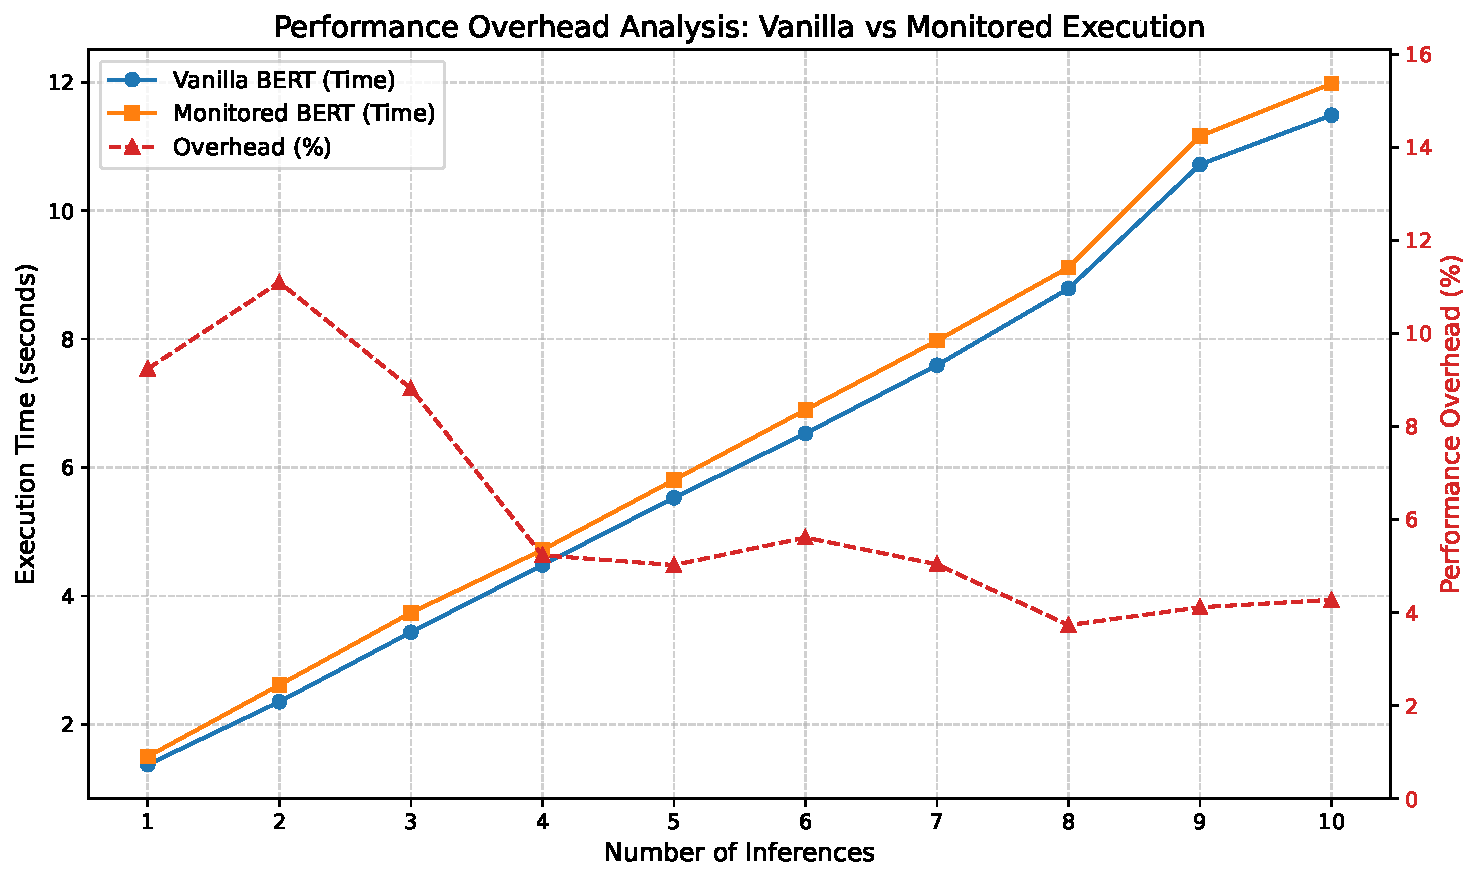
\includegraphics[width=0.45\textwidth]{figs/inference_overhead.pdf}
    \caption{Execution time of Vanilla vs.\ Monitored BERT and relative overhead across inferences.}
    \label{fig:inference_overhead}
\end{figure}


\textbf{Performance Overhead Analysis.} The performance impact of \toolname{} on normal model execution is presented in Table~\ref{tab:overhead_result}. \toolname{} introduces marginal overhead: the total execution time increases by an average of only 5.69\%, with the overhead consistently remaining within a narrow 4.9\% to 6.0\% margin across fundamentally different model architectures.

This performance penalty is attributed to our architectural design. First, the application-layer dynamic instrumentation employs a lightweight boundary-hooking mechanism that only captures high-level metadata instead of deeply traversing and serializing complex, multi-gigabyte Tensor objects. More importantly, the Autoencoder screening module and the \ac{llm} reasoning module run entirely asynchronously on the CPU. Because they do not compete for GPU memory or compute cycles, the intensive matrix multiplications and data parallelism required for AI inference remain completely unhindered.

To further demonstrate that our detection system minimally impacts inference efficiency, we analyzed the relationship between the number of inference iterations and relative latency overhead. Figure~\ref{fig:inference_overhead} illustrates the execution time of the BERT model over 1 to 10 inference steps, comparing vanilla execution with \toolname{}-monitored execution. The relative overhead percentage is highest during the initial executions but quickly drops and stabilizes at a lower baseline as the number of inferences increases.

This phenomenon aligns with the operating characteristics of deep learning frameworks. The model loading and initialization phases generate a large number of intensive system calls, such as memory mapping operations and heavy file I/O for loading model weights, which incur temporary CPU-bound monitoring overhead. However, once the model enters the continuous inference phase, intensive computations are primarily offloaded to hardware accelerators. These computations generate very few new system calls and do not occupy main CPU resources. Therefore, the overhead introduced by dynamic instrumentation and system call monitoring gradually diminishes.

\textbf{Detection Latency Analysis.} As shown in Table~\ref{tab:overhead_result}, \toolname{} achieves an average detection latency of 9.79 seconds. This latency encompasses the full analytical pipeline: capturing low-level system calls, completing the Autoencoder forward pass, extracting the corresponding Python contextual logs, and generating the final \ac{llm} intent classification. The \ac{llm} intent classification is only invoked on a small fraction of operations marked as abnormal by the Autoencoder, so its cost does not scale with total runtime but solely with the number of suspicious events.

While dynamic reasoning inherently introduces some delay compared to simple signature matching, this two-stage design keeps the overall overhead well within the acceptable budget for offline model vetting pipelines and pre-deployment security checks. 

\label{sec:rq3}

\subsection{RQ3: Component Ablation and Sensitivity}
In this section, we evaluate the contribution of each core component of \toolname{} through ablation studies. To demonstrate the necessity of our two-stage cross-layer architecture, we evaluate two variants:

\begin{itemize}
    \item \emph{\toolname{}--S}: which removes the unsupervised Autoencoder screening stage, directly feeding all raw system call windows and application-level instrumentation logs to the \ac{llm} for anomaly detection;
    \item \emph{\toolname{}--L}: which removes the application-level dynamic instrumentation, relying solely on the anomalous system call operations to make its final judgment;
\end{itemize}

\begin{table}[t!]
    \scriptsize
    \centering
    \caption{Ablation study of \toolname{}.}
    \resizebox{0.49\textwidth}{!}{\begin{tblr}{
        cell{1}{1-6} = {c},
        cell{2-4}{2-6} = {c},
        vline{2},
        hline{1,5} = {1pt},
        stretch=0
    }
    \SetCell[r = 1, c = 1]{c} \textbf{Method} & \SetCell[r = 1, c = 1]{c} \textbf{Precision} & \SetCell[r = 1, c = 1]{c} \textbf{Recall} & \SetCell[r = 1, c = 1]{c} \textbf{F1} & \SetCell[r = 1, c = 1]{c} \textbf{Latency (s)} & \SetCell[r = 1, c = 1]{c} \textbf{Token Cost} \\ \hline
    \SetCell[r = 1, c = 1]{c} \textbf{\toolname{}-S} & 90.91\% & 44.30\% & 59.57\% & 30.3126 & 867075 \\
    \SetCell[r = 1, c = 1]{c} \textbf{\toolname{}-L} & 85.25\%   & \textbf{98.99\%} & 91.61\% & \textbf{8.9778} & \textbf{50005} \\ \hline
    \SetCell[r = 1, c = 1]{c} \textbf{\toolname{}} & \textbf{100.00\%} & \textbf{98.99\%} & \textbf{99.49\%} & 9.7934 & 57207.1 \\
    \end{tblr} }
    \label{tab:ablation_metrics}
\end{table}


We evaluate these two variants and compare them with the full \toolname{} model. The evaluation metrics cover detection accuracy and system efficiency. Table~\ref{tab:ablation_metrics} details the comprehensive metrics.
Overall, both variants exhibit significantly degraded performance or unacceptable system overhead compared to the full model, proving that both stages are indispensable.

Specifically, \toolname{}-S suffers from a catastrophic decrease in detection efficiency and a massive surge in \ac{llm} token consumption. Because it bypasses the Autoencoder screening, the \ac{llm} is overwhelmed by the massive volume of benign, repetitive system events. This increases the average detection latency and incurs extreme API costs. It also slightly reduces precision, as the \ac{llm} is more prone to hallucination when processing excessive background noise. This demonstrates that the statistical screening stage is crucial for filtering out normal activity and maintaining practical deployability.

On the other hand, \toolname{}-L performs the worst in detection accuracy, particularly suffering a severe drop in precision. By removing the application-level instrumentation logs, the \ac{llm} is forced to judge intent based entirely on low-level system calls. Without high-level semantic context such as function arguments to explain why a system call was executed, benign operations are frequently misclassified as malicious. This confirms that dynamic cross-layer context alignment is an important component for eliminating false positives and accurately discerning the true intent of AI models.



